\section{AMP on Tadpole Graphs} \label{tadpoles}
In this section we cover multi-agent graph exploration on tadpole graphs. In \S\ref{lower_bound_tad} we show a lower bound of $1.5$ for the online exploration of tadpole graphs with $k\geq2$ agents in the time-, and $k=2$ agents in the energy model.
In \S\ref{tadpole_two} we show that random choice with two agents leads to a $2.5$-competitive strategy. In \S\ref{tadpole_three} we provide a modification of the \textit{AMP Algorithm} from \S \ref{cycles} that yields a competitive ratio of $1$ for the energy- and $2$ for the time model, 
using three agents. In \S\ref{tadpole_four} we describe an exploration strategy which matches the competitive lower bound of $1.5$ using $k=4$ agents. In Table \ref{table:tadpole} an overview of the results of this section is given.

    \begin{table}[H]
        \small
        \centering
        \begin{tabular}{|l|ll|ll|}
        \hline
                  & \multicolumn{2}{c|}{Time Model}                                     & \multicolumn{2}{c|}{Energy Model}                                   \\ \hline
                  & \multicolumn{1}{c|}{Lower Bound} & \multicolumn{1}{c|}{Upper Bound} & \multicolumn{1}{c|}{Lower Bound} & \multicolumn{1}{c|}{Upper Bound} \\ \hline
        1 Agent   & \multicolumn{1}{l|}{2 \cite{Brandt2020}}           & 2\cite{Brandt2020}                                & \multicolumn{1}{l|}{2\cite{Brandt2020}}           & 2\cite{Brandt2020}                               \\ \hline
        2 Agents  & \multicolumn{1}{l|}{1.5 (Thm. \ref{TadpoleTimeLower})}         & 2.5 (Thm. \ref{TadpoleUpperTwo})                              & \multicolumn{1}{l|}{1.5 (Thm. \ref{TadpoleEnergyLower})}            & 2.5 (Thm. \ref{TadpoleUpperTwo})                               \\ \hline
        3 Agents  & \multicolumn{1}{l|}{1.5 (Thm. \ref{TadpoleTimeLower})}         & 2 (Thm. \ref{TadpoleUpperThree})                               & \multicolumn{1}{l|}{1}           & 1 (Thm. \ref{TadpoleUpperThree})                               \\ \hline
        4+ Agents & \multicolumn{1}{l|}{1.5 (Thm. \ref{TadpoleTimeLower})}         & 1.5 (Thm. \ref{TadpoleUpperFour})                             & \multicolumn{1}{l|}{1}           & 1 (Thm. \ref{TadpoleUpperThree})                               \\ \hline
        \end{tabular}
        \caption{Results for multi-agent exploration of tadpole graphs.} \label{table:tadpole}
    \end{table}

\subsection{A lower bound for tadpole graphs}\label{lower_bound_tad}

In this section we show lower bounds for graph exploration on tadpole graphs. We first show that the exploration of any tadpole graph has a competitive ratio of at least
$1.5$ for $k\geq 2$ agents in the time model. For the energy model we show a lower bound of $1.5$ with $k=2$ agents. 
\subsubsection*{$k\geq2$ agents in the time model} We modify the graph construction Higashikawa et al.\ used to show the lower bound of $1.5$ for cycles with $2$ agents \cite{Higashikawa2012},
to show a lower bound of $1.5$ for the time model for tadpole graphs with $k \geq 2$ agents, by simply attaching a tail consisting of a single edge with of length $\varepsilon$ to the starting node $s$.
Note that the analysis stays basically identical to the analysis by Higashikawa et al.\ \cite{Higashikawa2012}, since in the offline case the tail can always be explored in parallel, having no impact on the
optimal exploration time.

\begin{theorem}[Time Model: Lower bound for exploring tadpole graphs]\label{TadpoleTimeLower}
    For any number of agents $k \geq 2$, any online exploration strategy for tadpole graphs has a competitive ratio of at least $1.5$ in the time model.
\end{theorem}

\begin{figure}[H]
    \begin{center}
    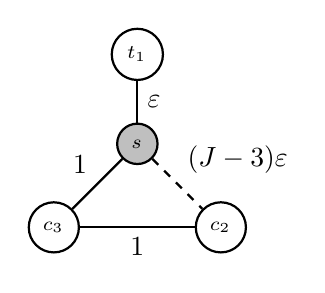
\begin{tikzpicture}[node distance={15mm}, thick, main/.style = {draw, circle}, scale=0.5] 
        \node[main, fill=gray!50, minimum size=0.5cm] (3) [] {$_{s}$ }; 
        \node[main, minimum size=0.5cm] (2) [below left of = 3] {$_{c_3}$ }; 
        \node[main, minimum size=0.5cm] (4) [below right of = 3] {$_{c_2}$ };
        \node[main, minimum size=0.5cm] (6) [above of = 3, above=-2em] {$_{t_1}$ };
        \draw (2) [] to node[below] {$1$} (4);
        \draw (2) [] to node[above left] {$1$} (3);
        \draw (3) [dashed] to node[above right] {$(J-3)\varepsilon$} (4);
        \draw (3) [] to node[right] {$\varepsilon$} (6);
    \end{tikzpicture} 
    \hspace*{5em}
    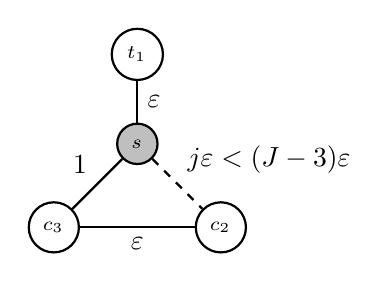
\begin{tikzpicture}[node distance={15mm}, thick, main/.style = {draw, circle}, scale=0.5] 
        \node[main, fill=gray!50, minimum size=0.5cm] (3) [] {$_{s}$ }; 
        \node[main, minimum size=0.5cm] (2) [below left of = 3] {$_{c_3}$ }; 
        \node[main, minimum size=0.5cm] (4) [below right of = 3] {$_{c_2}$ };
        \node[main, minimum size=0.5cm] (6) [above of = 3, above=-2em] {$_{t_1}$ };
        \draw (2) [] to node[below] {$\varepsilon$} (4);
        \draw (2) [] to node[above left] {$1$} (3);
        \draw (3) [dashed] to node[above right] {$j\varepsilon < (J-3)\varepsilon$} (4);
        \draw (3) [] to node[right] {$\varepsilon$} (6);
    \end{tikzpicture} 
    \end{center}
    \caption[Tadpole lower bound]{Any number of agents $k\geq2$ cannot explore the given graph with a competitive ratio lower than $1.5$. The dotted line is a path consisting entirely of edges with length $\varepsilon$.
    Case 1 (Left): the graph an adversary reveals if $(s, c_3)$ is not traversed after an agent traversed a distance of $(J-3)\varepsilon$ on the path between $s$ and $c_2$.
    Case 2 (Right): the graph an adversary creates when $(s,c_3)$ is traversed before an agent traverses a distance of $j\varepsilon<(J-3)\varepsilon$ on the path between $s$ and $c_2$.}
    \label{tadpole-time}
\end{figure}
\begin{proof}
    Consider the graphs shown in Figure \ref{tadpole-time}. In the beginning, the agents only see two edges of length $\varepsilon$ and one edge of length $1$. There are two cases depending on when an agent decides to 
    explore the edge $(s,c_3)$. Let $\varepsilon=\frac{1}{J}$ and $J \in \mathbb{N}$.
    \begin{enumerate}
        \item An agent traverses a distance of $(J-3)\varepsilon$ on $(s,c_2)$ before an agent enters the edge $(s,c_3)$.
        \item An agent starts traversing $(s,c_3)$ when a distance $j\varepsilon<(J-3)\varepsilon$ is traversed on $(s,c_2)$
    \end{enumerate}
    \paragraph*{Case 1} In this case the adversary sets $l(c_2, c_3)=1$. The optimal offline strategy would have sent one agent from $s$ to $c_3$ and back, while another agent in parallel explores the edge
    $(s,t_1)$ and the path $(s,c_2)$, resulting in an exploration time of $2$. The online strategy has already taken a time of at least $(1-3\varepsilon)$ and needs at least time $2$ to complete the exploration,
    leading to a minimum exploration time of $(3-3\varepsilon)$.
    \paragraph*{Case 2} In this case the adversary sets $l(c_2, c_3)=\varepsilon$ and lets $c_2$ be the next visited node by the searcher on the path from $s$ to $c_2$. 
    The optimal offline strategy would send one agent from $s$ to $c_3$ via $c_2$ and back, while another agent explores the tail in parallel, leading to an exploration time of $2(j+1)\varepsilon$. The online strategy
    has already traversed a distance of at least $(j-1)\varepsilon$ before an agent started traversing $(s,c_3)$. After reaching $c_3$ the fastest way to $s$ is traversing the graph via $c_2$. Since
    $1=J\varepsilon\geq (j+3)\varepsilon$, the entire exploration
    has at least length $(j-1)\varepsilon + (j+3)\varepsilon + (j+1)\varepsilon = 3(j+1)\varepsilon$.
\end{proof}
\subsubsection*{Two agents in the energy model} For showing $1.5$-competitiveness in the energy model, we modify the construction Dynia et al.\ used to show a lower bound of $1.5$ for the exploration
of trees \cite{Dynia2006}, to create a tadpole graph.

\begin{theorem}[Energy Model: Lower bound for exploring tadpole graphs]\label{TadpoleEnergyLower} 
    For $k=2$ agents, no online exploration strategy on tadpole graphs can have a competitive ratio better than $1.5$ in the energy model.
\end{theorem}

\begin{figure}[H]
    \begin{center}
    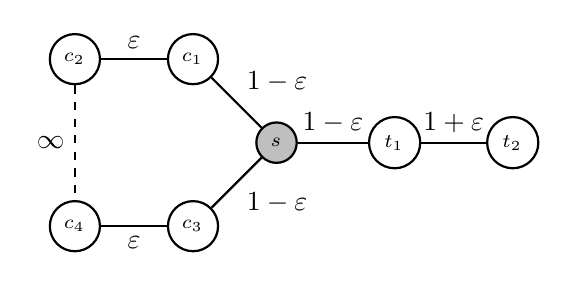
\begin{tikzpicture}[node distance={15mm}, thick, main/.style = {draw, circle}, scale=0.5] 
        \node[main, fill=gray!50, minimum size=0.5cm] (2) {$_{s}$ }; 
        \node[main, minimum size=0.5cm] (1) [above left of = 2] {$_{c_1}$ }; 
        \node[main, minimum size=0.5cm] (4) [left of = 1] {$_{c_2}$ }; 
        \node[main, minimum size=0.5cm] (3) [below left of = 2] {$_{c_3}$ };
        \node[main, minimum size=0.5cm] (5) [left of = 3] {$_{c_4}$ };  
        \node[main, minimum size=0.5cm] (6) [right of = 2] {$_{t_1}$ };
        \node[main, minimum size=0.5cm] (7) [right of = 6] {$_{t_2}$ };
        \draw (1) to node[above right] {$1-\varepsilon$} (2);
        \draw (2) to node[below right] {$1-\varepsilon$} (3);
        \draw (4) [dashed] to node[left] {$\infty$} (5);
        \draw (1) to node[above] {$\varepsilon$} (4);
        \draw (3) to node[below] {$\varepsilon$} (5);
        \draw (2) to node[above] {$1-\varepsilon$} (6);
        \draw (6) to node[above] {$1+\varepsilon$} (7);
    \end{tikzpicture} 
    \end{center}
    \caption[Lower Bound Energy Model]{Lower Bound construction for the energy model.}
    \label{fig:energybound}
\end{figure}

\begin{proof}
    Let $\varepsilon > 0$ be an arbitrary small and $\infty$ be an arbitrary large number.
    Consider the graph shown in Figure \ref{fig:energybound}. An optimal offline solution starting at $s$ would send one agent from $s$ to $t_2$ and back, while the other agent
    simultaneously explores the cycle, traversing each edge except $(c_2, c_4)$ twice, leading to a maximum distance of $4$ traversed by any agent.\\
    In the online case the agents cannot distinguish the edges they see when starting at $s$. Since $c_2$ and $c_4$ are hidden behind edges of length $\varepsilon$, the remaining two
    paths cannot be distinguished even if one agent has already traversed a path from $s$ to $c_2$ or $c_4$. Because of this an adversary could always affect the exploration
    order of the two agents, so that the maximum distance traversed by any agent is at least $6-2\varepsilon$. This leads to a competitive ratio of $1.5$ for arbitrary small $\varepsilon$.
\end{proof}

\subsection{Tadpole graphs with two agents}\label{tadpole_two}

We construct a $2.5$ competitive exploration strategy by using two agents for the exploration of a tadpole graph, where random paths are chosen as soon as the intersection is found.


    \begin{theorem}[Upper bound for two-agent randomized tadpole graph exploration]\label{TadpoleUpperTwo}
        Using the \textit{AMP} strategy with two agents for the exploration of tadpole graphs, choosing random paths as soon as the intersection is found,
        leads to a competitive upper bound of $2.5$ compared to an optimal offline strategy using two agents.
    \end{theorem}
    

\begin{proof} Consider how an online strategy exploring tadpole graphs can distinguish 3 cases for the start of an exploration: If the degree of the starting node $s$ is 1,
    it must be the end of the tail, if the degree is 3, it must be the intersection $v_i$. If starting node has degree 2, it can be any other node of the graph.
    The possible starting positions for an exploration are depicted in Figure \ref{Tail}.
    We describe the exploration strategies for each of these starting positions and show that for any of those, an online strategy choosing
    a random direction when finding the intersection, takes at most time $5\max(d(s,v), v\in \{v_\ell, v_t\})$ for the exploration of any tadpole graph. 
    Since any optimal strategy takes at least time $2\max(d(s,v), v\in \{v_\ell, v_t\})$ to explore any tadpole graph, this directly leads to a competitive
    upper bound of $2.5$. We then provide an example, in which our strategy takes $2.5$ times the optimal exploration time.

    \begin{figure}[H]
        \begin{center}
        \adjustbox{max width=\textwidth}{
        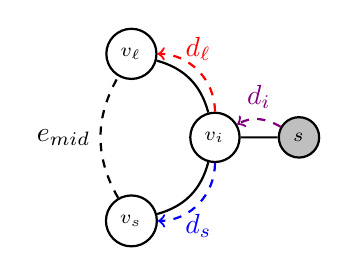
\begin{tikzpicture}[node distance={15mm}, thick, main/.style = {draw, circle}, scale=0.3]
            \node[main, minimum size=0.5cm] (2) {$_{v_s}$ }; 
            \node[main, minimum size=0.5cm] (3) [above right of = 2] {$_{v_i}$ }; 
            \node[main, minimum size=0.5cm] (4) [above left of = 3] {$_{v_\ell}$ };
            \node[main, fill=gray!50, minimum size=0.5cm] (6) [right of = 3, right=-2em] {$_{s}$ };
            \draw (2) [bend left, dashed] to node[left] {$e_{mid}$} (4);
            \draw (2) [bend right] to node[right] {} (3);
            \draw (3) [bend right] to node[above right] {} (4);
            \draw (3) [] to node[above] {} (6);
            \path [red, thick, dashed, ->] (3) edge[out=90,in=0] node[above] {{$d_\ell$}} (4);
            \path [blue, thick, dashed, ->] (3) edge[out=270,in=0] node[below] {{$d_s$}} (2);
            \path [violet, thick, dashed, ->] (6) edge[out=150,in=30] node[above] {{$d_i$}} (3);
        \end{tikzpicture} 
        \hspace*{1em}
        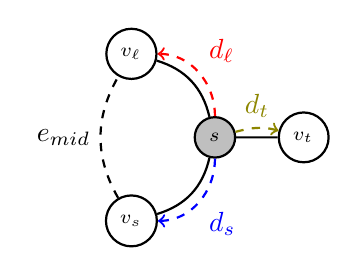
\begin{tikzpicture}[node distance={15mm}, thick, main/.style = {draw, circle}, scale=0.3] 
            \node[main, minimum size=0.5cm] (2) {$_{v_s}$ }; 
            \node[main, fill=gray!50, minimum size=0.5cm] (3) [above right of = 2] {$_{s}$ }; 
            \node[main, minimum size=0.5cm] (4) [above left of = 3] {$_{v_\ell}$ };
            \node[main, minimum size=0.5cm] (6) [right of = 3, right=-2em] {$_{v_t}$ };
            \draw (2) [bend left, dashed] to node[left] {$e_{mid}$} (4);
            \draw (2) [bend right] to node[right] {} (3);
            \draw (3) [bend right] to node[above right] {} (4);
            \draw (3) [] to node[above] {} (6);
            \path [red, thick, dashed, ->] (3) edge[out=90,in=0] node[above right] {{$d_\ell$}} (4);
            \path [blue, thick, dashed, ->] (3) edge[out=270,in=0] node[below right] {{$d_s$}} (2);
            \path [olive, thick, dashed, ->] (3) edge[out=15,in=165] node[above] {{$d_t$}} (6);
        \end{tikzpicture} 
        \hspace*{1em}
        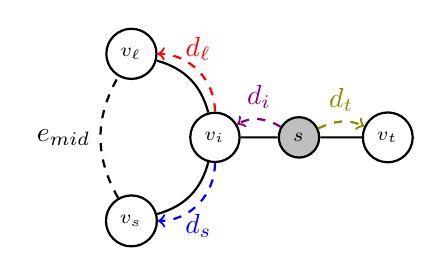
\begin{tikzpicture}[node distance={15mm}, thick, main/.style = {draw, circle}, scale=0.3] 
            \node[main, minimum size=0.5cm] (2) {$_{v_s}$ }; 
            \node[main, minimum size=0.5cm] (3) [above right of = 2] {$_{v_i}$ }; 
            \node[main, minimum size=0.5cm] (4) [above left of = 3] {$_{v_\ell}$ };
            \node[main, fill=gray!50, minimum size=0.5cm] (6) [right of = 3, right=-2em] {$_{s}$ };
            \node[main, minimum size=0.5cm] (5) [right of = 6, right=-2em] {$_{v_t}$ }; 
            \draw (2) [bend left, dashed] to node[left] {$e_{mid}$} (4);
            \draw (2) [bend right] to node[right] {} (3);
            \draw (3) [bend right] to node[above right] {} (4);
            \draw (3) [] to node[above] {} (6);
            \draw (6) [] to node[above] {} (5);
            \path [red, thick, dashed, ->] (3) edge[out=90,in=0] node[above] {{$d_\ell$}} (4);
            \path [blue, thick, dashed, ->] (3) edge[out=270,in=0] node[below] {{$d_s$}} (2);
            \path [violet, thick, dashed, ->] (6) edge[out=150,in=30] node[above] {{$d_i$}} (3);
            \path [olive, thick, dashed, ->] (6) edge[out=25,in=155] node[above] {{$d_t$}} (5);
        \end{tikzpicture} 
        \hspace*{1em}
        \begin{tikzpicture}[node distance={15mm}, thick, main/.style = {draw, circle}, scale=0.3] 
            \node[main, minimum size=0.5cm] (2) {$_{v_i}$}; 
            \node[main, fill=gray!50, minimum size=0.5cm] (5) [below left of = 4] {$_{s}$ }; 
            \node[main, minimum size=0.5cm] (3) [above right of = 2] {$_{v_\ell}$ }; 
            \node[main, minimum size=0.5cm] (4) [above left of = 3] {$_{v_s}$ };
            \node[main, minimum size=0.5cm] (6) [below of = 2] {$_{v_t}$ };
            \draw (2) [bend left] to node[left] {} (5);
            \draw (5) [bend left] to node[left] {} (4);
            \draw (2) [bend right] to node[right] {} (3);
            \draw (3) [bend right, dashed] to node[right] {$e_{mid}$} (4);
            \draw (2) [] to node[above] {} (6);
            \path [blue, thick, dashed, ->] (5) edge[out=90,in=180] node[left] {{$d_s$}} (4);
            \path [red, thick, dashed, ->] (5) edge[looseness=1.2,out=320,in=220] node[above] {{$d_\ell$}} (3);
            \path [olive, thick, dashed, ->] (2) edge[out=315,in=45] node[right] {{$d_t$}} (6);
            \path [violet, thick, dashed, ->] (5) edge[out=270,in=180] node[left] {{$d_i$}} (2);
        \end{tikzpicture} 
        }
        \end{center}
        \caption[Case1]{The possible starting positions in a tadpole graph.}
        \label{Tail}
    \end{figure}

\paragraph*{Starting at the end of the tail}

When starting at the end of the tail, both agents can be sent to the intersection, explore the cycle using an optimal $1.5$-competitive strategy
and return to $s$. This also leads to a $1.5$-competitive strategy. Since the paths taken to explore the cycle are identical to an optimal exploration,
this case is also $1$-competitive in the energy model.

\begin{align*}
    \opt &= 2d_t + \opt_C\\
    \onl &\leq 2d_t + 1.5\opt_C \leq 1.5\opt
\end{align*}

\paragraph*{Starting at the intersection}

When starting on the intersection, we randomly choose two outgoing edges and have each agent follow one path while applying the AMP strategy.
There are three possibilities for the paths chosen: $p_s$ and $p_\ell$, $p_s$ and $p_t$, or $p_\ell$ and $p_t$.\\
When $p_s$ and $p_\ell$ are chosen, which means exploring the cycle first, the agents explore the cycle and return. 
The first agent reaching $s$ again (which is the one that traversed $p_s$) will then explore the tail of the graph. 
This leads to a maximum exploration time of $d_s + d_\ell + \max(d_s+2d_t, d_\ell) \leq 5\max(d_\ell, d_t)$.\\

When $p_\ell$ and $p_t$ are chosen, one agent explores the tail, while another agent starts exploring the cycle. When the cycle is fully explored,
before the end of the tail is reached, the remaining agent then explores the rest of the tail and returns to $s$, leading to an exploration time less than
$3d_t \leq 5\max(d_\ell, d_t)$. If the end of the tail is reached before the cycle is fully explored, the agent exploring $p_t$ returns to $s$ and starts
exploring the remaining path $p_s$. When $d_t < d_\ell + l(e_{mid})$, the entire exploration time is at most $2d_t + 2d_\ell + d_s \leq 5\max(d_\ell, d_t)$.
If $d_t \geq d_\ell + l(e_{mid})$, the entire exploration time is at most $3d_t + 2d_s \leq 5\max(d_\ell, d_t)$. When choosing $p_s$ and $p_t$ we get 
exploration times of at most $3d_t$ (when $L \leq d_t$), $2d_t + 2d_\ell + d_s$ (when $d_t < d_s$), or $3d_t + 2d_\ell$ (when $d_t \geq d_s + l(e_{mid})$),
which are all less or equal to $5\max(d_\ell, d_t)$


\paragraph*{Starting on a node from the tail}

When starting on a node from the tail, one agent starts traversing in each direction, following the AMP strategy. When the intersection is found by
some agent, it randomly chooses an outgoing path. This leads to two possibilities: $p_t, p_\ell$ and $p_t, p_s$. In both cases, if $d_t \geq d_i + L$,
the exploration takes at most time $3d_l$. When $p_t$ and $p_\ell$ are chosen and $p_t \geq d_i + d_\ell + l(e_{mid})$, the exploration time is at most 
$3d_t + 2d_i + 2d_s$. If $p_t < d_i + d_\ell + l(e_{mid})$, the exploration takes at most time $2d_t + 3d_i + 2d_\ell + d_S$. When $p_t$ and $p_s$ are chosen
the exploration times are $3d_t + 2d_i + 2d_\ell$ (if $p_t \geq d_i + d_s + l(e_{mid})$) and $2d_t + 3d_i + 2d_\ell + d_S$ (if $p_t < d_i + d_s + l(e_{mid})$) respectively.

\paragraph*{Starting on a node from the cycle}

When starting on the cycle, there are two possibilities: $v_i$ can be located on either $p_s$ or $p_\ell$. In both cases the combination $p_\ell, p_s$ can be chosen,
which leads to maximum exploration times of $d_\ell + d_s + \max(d_s, d_\ell + 2d_t)$ (when $v_i$ is on $p_\ell$), or $d_\ell + d_s + \max(d_\ell, d_s + 2d_t)$ (when $v_i$ is on $p_s$).
We now cover the remaining cases: When $v_i$ is on $p_s$ and $p_\ell, p_t$ are chosen and $d_i + d_t \geq L - d_i$, meaning that the cycle is fully
explored before $v_t$ is reached, the exploration takes time at most $2(d_i + d_t)$. If $d_i + d_t < d_\ell + l(e_{mid})$, the exploration takes time $2d_t + 2d_\ell + d_s$.
If $d_i + d_t \geq d_\ell + l(e_{mid})$ the exploration takes time at most $3d_t + 2d_s + d_i$. When $v_i$ is on $p_\ell$ the exploration times are 
$2(d_i + d_t)$ (if $d_i + d_t \geq L - d_i$), $2d_t + 2d_\ell + d_s$ (if $d_i + d_t < d_s + l(e_{mid})$) and $3d_t + 2d_\ell + d_i$ (if $d_i + d_t \geq d_s + l(e_{mid})$) respectively.


\begin{figure}[H]
    \begin{center}
        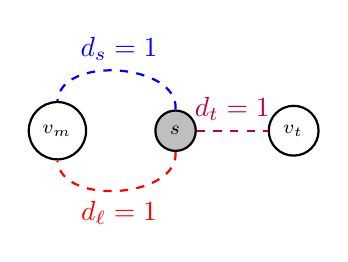
\begin{tikzpicture}[node distance={15mm}, thick, main/.style = {draw, circle}] 
            \node[main, fill=gray!50, minimum size=0.5cm] (3) [] {$_{s}$ }; 
            \node[main, minimum size=0.5cm] (4) [left of = 3] {$_{v_m}$ };
            \node[main, minimum size=0.5cm] (6) [right of = 3] {$_{v_t}$ };
            \draw (3) [color=blue, dashed, bend right, out=270, in=270] to node[above] {$d_s = 1$} (4);
            \draw (3) [color=red, dashed, bend left, out=90, in=90] to node[below] {$d_\ell = 1$} (4);
            \draw (3) [color=purple, dashed] to node[above] {$d_t = 1$} (6);
        \end{tikzpicture} 
    \end{center}
    \caption[Tadpole example]{An example of a tadpole graph, where the competitive ratio can reach $2.5$. The dashed lines are paths with edges of length $\varepsilon$.
     If two agents randomly choose $d_s, d_\ell$ at the start of the exploration, the online exploration time reaches $5$, while the optimal exploration time with two agents is $2$.}
    \label{Example_randomchoice}
\end{figure}

\paragraph*{Example in which a competitive ratio of exactly $2.5$ is reached}

Figure \ref{Example_randomchoice} depicts a graph in which the described exploration strategy reaches a competitive ratio of exactly $2.5$, if $p_s$ and $p_\ell$ are chosen at the
start of the exploration. In this case the cycle is explored, with the agents meeting at $v_{mid}$, before the agents backtrack to $s$ and then explore the tail of the graph. The exploration time 
is $5$. An optimal strategy would have sent one agent to $v_t$ and back, while the other agent explores the cycle, leading to an exploration time of $2$.
\end{proof}

\subsection{Tadpole Graphs with three Agents}\label{tadpole_three}
We modify the \textit{AMP} algorithm from \S\ref{cycles}, to construct a strategy for exploring tadpole graphs with $k=3$ agents. 
In the following, we first describe this strategy and then show that it achieves an optimal competitive ratio of $1$ for the energy model
as well as a competitive ratio of $2$ for the time~model.


\begin{theorem}[Three agent tadpole graph exploration]\label{TadpoleUpperThree}
    For $k=3$ agents there exists an exploration strategy for tadpole graphs, which has a competitive ratio of $2$ for the time model, and $1$ for the energy model.
\end{theorem}

\begin{proof}
Similar to the proof of Thm.\ref{TadpoleUpperTwo} we show that the competitive ratios stated above hold for each possible starting position
in a tadpole graph when using three agents. Since a strategy with two agents already optimally explores the graph when starting on $v_t$,
we can focus on the remaining cases: $s = v_i$ and $s$ is a node with degree two.

\paragraph*{Starting on the intersection} 
When the starting node $s$ is the intersection, an exploration strategy can send one agent in each direction. Like in the \textit{AMP} strategy for cycles, only one
agent traverses an edge at a time, minimizing the maximum distance each agent has traversed from $s$ to its current position. Because of this, the cycle is explored
optimally for the energy model, with the agents following exactly the same paths as in the \textit{AMP} algorithm for cycles. The tail is also optimally explored for
the energy model, since the agent exploring the tail can only follow the same path as an agent would in an offline strategy, leading to a competitive ratio of $1$ for the energy model.
For the time model, we reach a competitive ratio of $2$, because the strategy takes time $d_t + d_\ell + d_s + \max(d_t,d_\ell) \leq 4\max(d_t,d_\ell)$, since only one agent moves
at a time until the graph is explored, before all agents return to $s$ in parallel.

\paragraph*{Starting on a node with degree two}
When starting on a node with degree two, one agent waits at the node $s$ until the intersection is found, while the other two agents use the \textit{AMP} strategy to
explore the graph in both directions. As soon as the intersection $v_i$ is discovered, the third agent moves to the intersection, while the other agents wait. When the third agent has reached the intersection,
all three agents explore the graph in different directions, following the \textit{AMP} strategy. Since the agent discovering the intersection takes the shortest path with length $d_i$, 
and the agents proceed as in case 2, the strategy still reaches a competitive ratio of $1$ for the energy model, as well as $2$ for the time model. When the agents start on the cycle, they
traverse a distance of $d_s + d_\ell + (d_i + d_t) + \max(d_i + d_t, d_\ell) \leq 4\max(d_i + d_t, d_\ell)$. When the agents start on the tail, they traverse a distance of 
$(d_i + d_s) + (d_i + d_\ell) + d_t + \max(d_t, d_i + d_\ell) \leq 4\max(d_t, d_i + d_\ell)$.
\end{proof}

\subsection{Tadpole Graphs with four Agents}\label{tadpole_four}

When using four agents to explore a tadpole graph, we can achieve a $1.5$-competitive exploration strategy for the time model,
as well as a $1$-competitive strategy for the energy model. Since the optimal offline strategy cannot yield a better result than $2\max(d(s,v)), v\in V$,
we can still use the strategy given in \S\ref{tadpole_three} to reach $1$-competitiveness for the energy model. Also, since the lower bound for the exploration of 
tadpole graphs is $1.5$ as shown in \S\ref{lower_bound_tad}, using more than four agents for the exploration cannot yield a better competitive ratio than this strategy.


\begin{theorem}[Exploring tadpole graphs with four agents]\label{TadpoleUpperFour}
    Using $k=4$ agents, a competitive ratio of $1.5$ can be achieved on tadpole graphs in the time model.
\end{theorem}


\begin{proof}
    Since the optimal offline strategy needs $2\max(d(s,v), v\in V)$ time to explore a tadpole graph, and our strategy needs time $\max(d(s,v), v\in V)$ to backtrack after
    the last node has been visited, we can show that our online strategy needs at most time $2\max(d(s,v), v\in V)$ until all nodes of the graph have been visited, to achieve a competitive
    ratio of $1.5$ for the entire exploration.\\
    When the agents start the exploration on the intersection, three agents are sent into the graph, one in each possible direction. If they start on a node with degree two, pairs of 
    two agents (behaving like a single agent, making all steps in parallel) are sent to both directions. As soon as the intersection is found by a pair of agents, it splits, so that at 
    least one agent is exploring each path.\\
    The agents start the exploration by comparing the entire traversed distance after adding the next edge, like in the AMP strategy, but in this case all agents but the
    one with the longest total traversed distance are moving. When two agents would have traversed the same distance, both agents move. Whenever some agent reaches a node, if another agent is currently waiting, they compare the distances after the next edge
    traversals and the one seeing a shorter distance immediately starts traversing the next edge, so that at most one agent is waiting at any point in time.\\
    Since the agents on all other currently visible paths are moving forward whenever some agent $a_k$ waits, the maximum time needed until it traverses a distance of $d_k$ is $(d_k + t) \leq 2d_k$,
    where $t$ is the time waited. This is the case because as soon as $a_k$ has waited for a time $t=d_k$, the other agents must have either traversed a distance of $d_k$, 
    or already finished their exploration, which leads to $a_k$ starting the traversal until it reaches the same distance without stopping.\\
    Since the agents are exploring the graph on all possible paths, each node $v\in V$ is reached by some agent after at most time $2d(s, v)$ has passed. Because of this the last visited node 
    is reached by some agent after at most time $2\max(d(s,v), v\in V)$ has passed.
\end{proof}
